\chapter{Perancangan}
\label{chap:perancangan}
Bab ini akan menjelaskan perancangan aplikasi visualisasi data histori KIRI pada google map

\section{Perancangan Antarmuka}
\label{sec:perancanganAntarmuka}
Pada aplikasi, disediakan antarmuka untuk memudahkan pengguna dalam berinteraksi dengan perangkat lunak \ref{fig:antarmuka}.

\begin{figure}[H]
	\centering  
	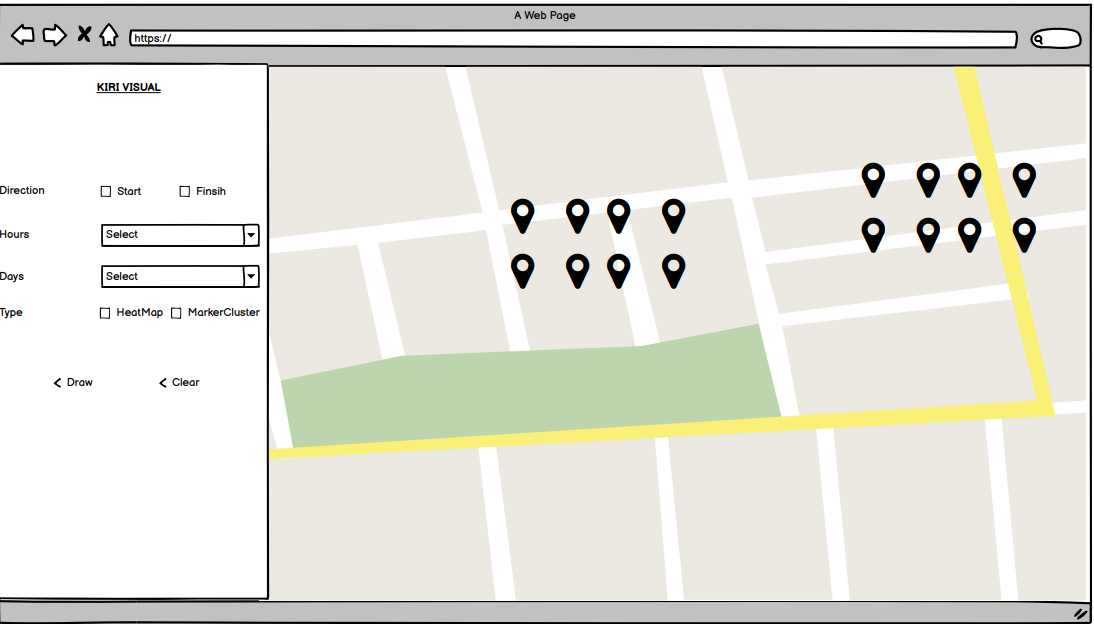
\includegraphics[scale=0.5]{Gambar/mockup.PNG}  
	\caption[Rancangan Antarmuka]{Rancangan Antarmuka} 
	\label{fig:antarmuka} 
\end{figure}

Berdasarkan rancangan diatas, berikut adalah fungsi dari setiap komponen dalam antarmuka:
\begin{itemize}
	\item \textit{Map}: digunakan untuk menampilkan peta \textit{google map}.
	\item \textit{Checkbox Start}:untuk memfilter data berdasarkan tempat keberangkatan.
	\item \textit{Checkbox End} :untuk memilfter data berdasarkan tempat tujuan.
	\item \textit{Selection Box Hours} : untuk memfilter data berdasarkan jam.
	\item \textit{Selection Box Days} : untuk memfilter data berdasarkan hari.
	\item \textit{Checkbox Heat Map} : untuk menampilkan data dalam bentuk \textit{heat map}.
	\item \textit{Checkbox Marker Clustering} : untuk menampilkan data dalam bentuk \textit{marker clustering}.
	\item Button \textit{Draw}: menampilkan data yang telah diolah kedalam objek \textit{map}.
	\item Button \textit{Clear}: menghapus seluruh \textit{overlay} pada objek \textit{map}.
\end{itemize}

\section{Perancangan Masukan dan Keluaran}
Aplikasi agregasi yang dibangun menggunakan antarmuka yang sudah dirancang seperti pada gambar \ref{fig:antarmuka}. Dapat diketahui masukan pada aplikasi ini berupa \textit{click} dari tombol dan \textit{selection box} yang tersedia dimana ketika tombol-tombol tersebut ditekan maka akan memfilter data histori KIRI. Keluaran dari aplikasi ini berupa visualsisai data histori KIRI pada objek \textit{map}.


\section{Perancangan Kelas Aplikasi Visualisasi Data Histori KIRI}
Pada subbab ini akan dijelaskan kelas diagram secara detail setelah sebelumnya dijelaskan diagram kelas sederhana pada subbab \ref{subsec:diagramKelas}. 

\subsection{Diagram Kelas Perangkat Lunak}
Pada penelitian ini dibuat satu diagram kelas lengkap, yaitu diagram kelas untuk perangkat lunak Visualisasi data histori KIRI.


\begin{figure}[H]
	\centering  
	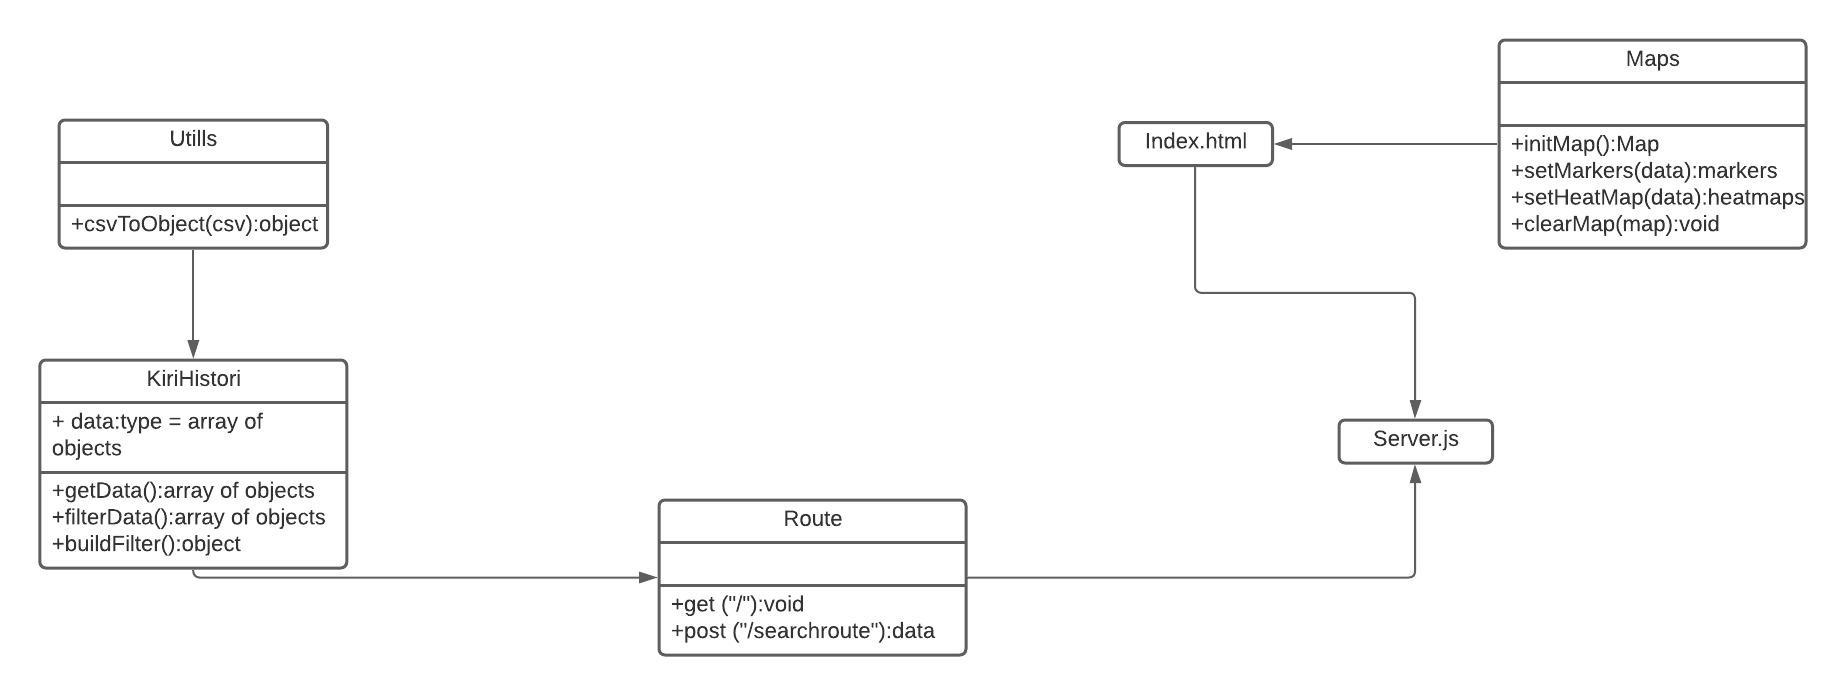
\includegraphics[scale=0.5]{Gambar/ClassDiagramLengkap.jpeg}  
	\caption[Rancangan Diagram Kelas]{Rancangan Diagram Kelas} 
	\label{fig:diagramKelas} 
\end{figure}

\subsection{Detil Setiap Kelas}

\begin{itemize}
    \item \textbf{Kelas KIRIHistori}
    \begin{figure}[H]
        	\centering  
        	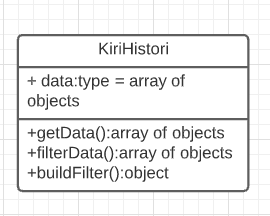
\includegraphics[scale=1]{Gambar/KIRI-Histori-Class.PNG}  
        	\caption[Kelas KIRI HISTORI]{Kelas KIRI HISTORI} 
        	\label{fig:KIRIHistoriClass} 
    \end{figure}
    kelas ini berfungsi sebagai kelas model yang berfungsi untuk mengolah data histori KIRI. Berikut ini adalah atribut-atribut yang dimiliki kelas ini adalah:
    \begin{itemize}
        \item data  atribut ini adalah atribut yang akan menampung data histori kiri
    \end{itemize}
    Kelas KIRIHistori juga memiliki \textit{function-function} seperti:
    \begin{itemize}
        \item getData adalah fungsi yang akan menjadi getter untuk atribut data
        \item filterData adalah fungsi yang akan melakukan perintah filter 
        \item buildFilter adalah fungsi yang akan membuat filter query
    \end{itemize}
    \item \textbf{Kelas Utils}
    \begin{figure}[H]
        	\centering  
        	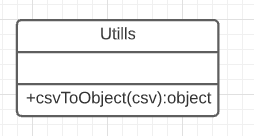
\includegraphics[scale=1]{Gambar/Utils-Class.PNG}  
        	\caption[Kelas Utils]{Kelas utils} 
        	\label{fig:utilsClass} 
    \end{figure}
    Kelas ini berfungsi sebagai kelas yang menyediakan \textit{function - function} tambahan untuk kelas KIRIHistori. Kelas ini memiliki \textit{function}:
    \begin{itemize}
        \item csvToObject \textit{function} ini akan menerima parameter csv data dan akan mengolah nya menjadi javascript objek
    \end{itemize}
    \item \textbf{Route}
        \begin{figure}[H]
        	\centering  
        	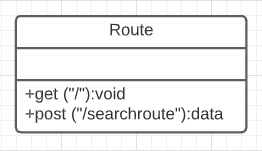
\includegraphics[scale=1]{Gambar/Route-Class.PNG}  
        	\caption[Kelas Route]{Kelas Route} 
        	\label{fig:routeClass} 
    \end{figure}
    Kelas ini berfungsi untuk mengatur \textit{route path} pada aplikasi visualisasi data histori KIRI. Pada kelas ini akan terdapat dua route yaitu:
    \begin{itemize}
        \item route get ("/") route ini akan mengembalikan tampilan yang akan dirender pada halaman utama
        \item route post ("/searhroute") route ini akan mengembalikan data histori yang telah difilter
    \end{itemize}
    \item \textbf{Server.js}
    \begin{figure}[H]
        	\centering  
        	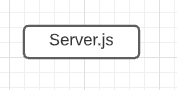
\includegraphics[scale=1]{Gambar/Server-Class.PNG}  
        	\caption[Kelas Server]{Kelas Server} 
        	\label{fig:serverClass} 
    \end{figure}
    Kelas ini akan menjadi kelas utama yang akan melakukan \textit{server side} rendering pada perangkat lunak ini.
    
    \item \textbf{Maps}
        \begin{figure}[H]
        	\centering  
        	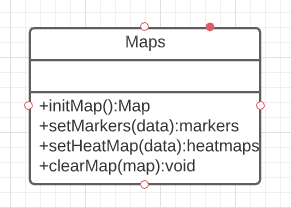
\includegraphics[scale=1]{Gambar/Maps-Class.PNG}  
        	\caption[Kelas Maps]{Kelas Maps} 
        	\label{fig:mapClass} 
    \end{figure}
    Kelas ini akan menjadi kelas yang menerima input data histori dan menampilkannya menggunakan \textit{google maps javascript api}.
    Pada kelas ini terdapat \textit{function - function} yaitu:
    \begin{itemize}
        \item initMap \textit{function} ini akan melakukan insiasi pada objek \textit{map}
        \item setHeatMap \textit{function} ini akan mengolah data histori kiri menjadi objek \textit{heat map}  agar dapat divisualisasikan pada objek \textit{map}
        \item setMarkers \textit{function} ini akan mengolah data histori kiri menjadi objek \textit{marker} agar dapat divisualisasikan pada objek \textit{map} 
    \end{itemize}

    \item \textbf{index}
           \begin{figure}[H]
        	\centering  
        	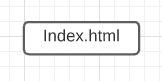
\includegraphics[scale=1]{Gambar/Index.PNG}  
        	\caption[Index]{Index} 
        	\label{fig:index} 
    \end{figure}
    Kelas ini akan menjadi kelas yang menampilkan tampilan utama pada perangkat lunak ini.
\end{itemize}

\section{Perancangan Pseudocode Aplikasi Visualisasi data histori KIRI}
Pada subbab ini dirancang \textit{pseudocode} untuk membuat aplikasi visualisasi data histori KIRI. Pada perangkat lunak ini akan dijelaskan psudocode pada kelas-kelas KIRIHistori , Utils , Route , Server , Maps



\subsection{Utils}
Kelas ini merupakan kelas yang akan memberikan \textit{function-function} bantuan untuk kelas KIRIHistori.
Pada kelas ini terdapat \textit{function} \texttt{csvToObject} yang akan berfungsi untuk mengolah data histori KIRI 
\begin{algorithm}[H]
\caption{csvToObject}
\label{psudo:constructorKIRIHistori}
    \begin{algorithmic}[1]
        \STATE $cols \leftarrow csv \rightarrow split('/')$
        \STATE $action \leftarrow cols[3]$
        \IF{$action == FINDROUTE$}
                \STATE $startLng \leftarrow cols[5]\rightarrow split("/")[0]$
                \STATE $endLat \leftarrow cols[5]\rightarrow split("/")[1]$
                \STATE $fullDate \leftarrow cols[2]$
                \RETURN ${object}$
       \ENDIF
    \end{algorithmic}
\end{algorithm}


\subsection{KIRIHistori}
Pada kelas ini terdapat \textit{constructor} yang akan meload data menggunakan \textit{javascript file system} pseudocode \textit{constructor} ini akan berupa
\begin{algorithm}[H]
\caption{Constructor KIRIHistori}
    \begin{algorithmic}[1]
        \STATE $data \leftarrow array \rightarrow map(csvToObject(item))$
    \end{algorithmic}
\end{algorithm}

% Kelas ini juga akan menyediakan \textit{function filter} yang akan berguna memfilter data berdasarkan \textit{input} dari pengguna.
% \begin{algorithm}[H]
% \caption{filtter}
%     \begin{algorithmic}[1]
%         \STATE $data \leftarrow array \rightarrow filter(query)$
%     \end{algorithmic}
% \end{algorithm}